\subsection{Bestimmung der Leerlaufspannung und Berechnung des Innenwiderstands für drei Spannungsquellen}
Die Ableseungenauigkeit der Stommessung beträgt $2 \% $ und die der Spannungsmessung $3 \% $. In den folgenden Diagrammen sind diese Fehler durch Fehlerbalken gekennzeichnet. \\
Mit einer linearen Regression mittels Python nach Formel \eqref{Klemmspannung}, folgen für die Monozelle die Leerlaufspannung
\[U_0 = \SI{1.471(14)}{\volt}\]
und der Innenwiderstand
\[\label{Innenwiderstand_Monozelle}
R_i = \SI{5.46(14)}{\ohm} \ .\]
\begin{figure}[h!]
	\centering
	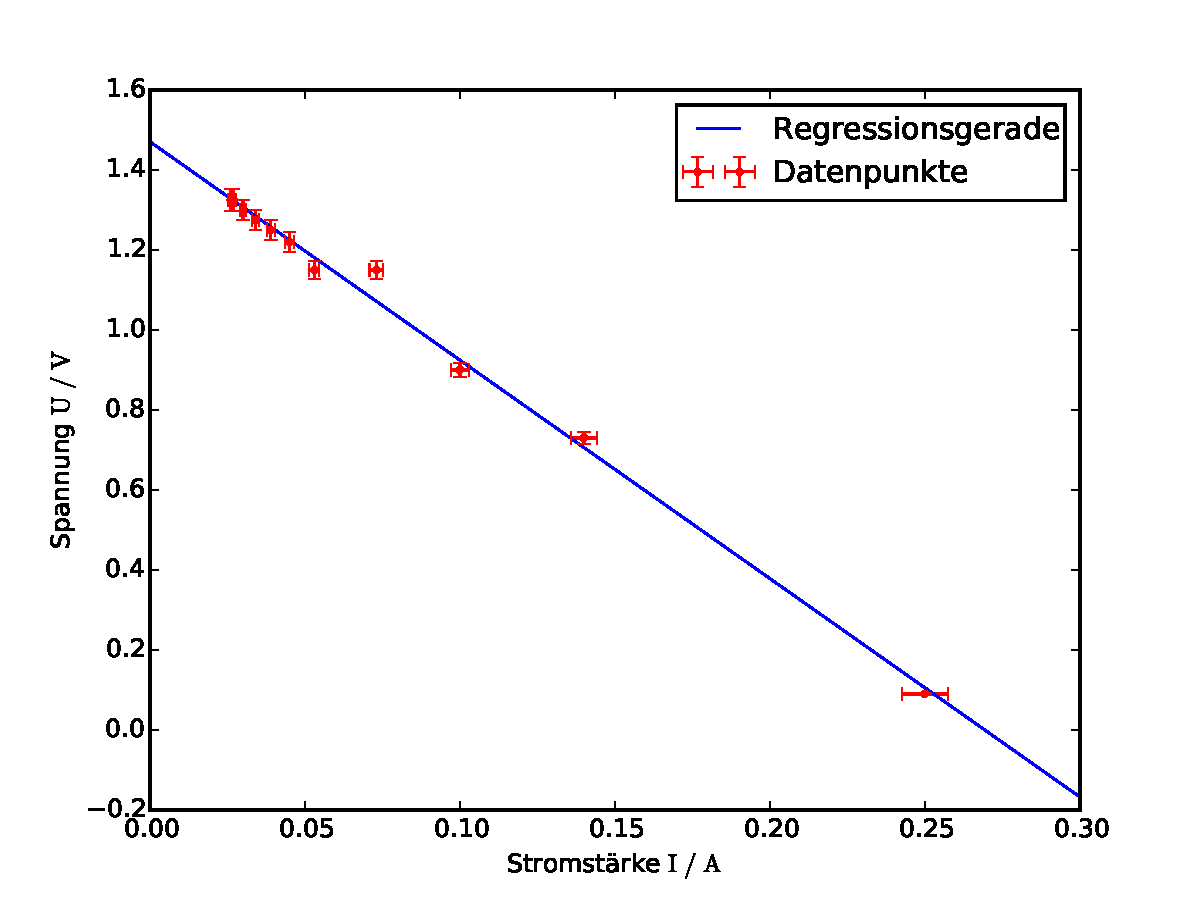
\includegraphics[width=0.95\textwidth]{Spannung_Messung_b.pdf}
	\caption{Lineare Regression zur Monozelle}
	\label{fig:Regression_Monozelle}
\end{figure}


Beim Anlegen der Gegenspannung (Abbildung \ref{Klemmspannung_Gegenspannung}) fließt der Strom in die entgegengesetzte Richtung, wodurch Formel \eqref{Klemmspannung} zu
\begin{equation}
U_k = IR_a = U_0+IR_i
\end{equation}
wird. Die lineare Regression liefert in diesem Fall :
\begin{align}
&U_0 = \SI{1.383(33)}{\volt} \ , \\
&R_i = \SI{5.91(24)}{\ohm}  \ .
\end{align}
\begin{figure}[h!]
	\centering
	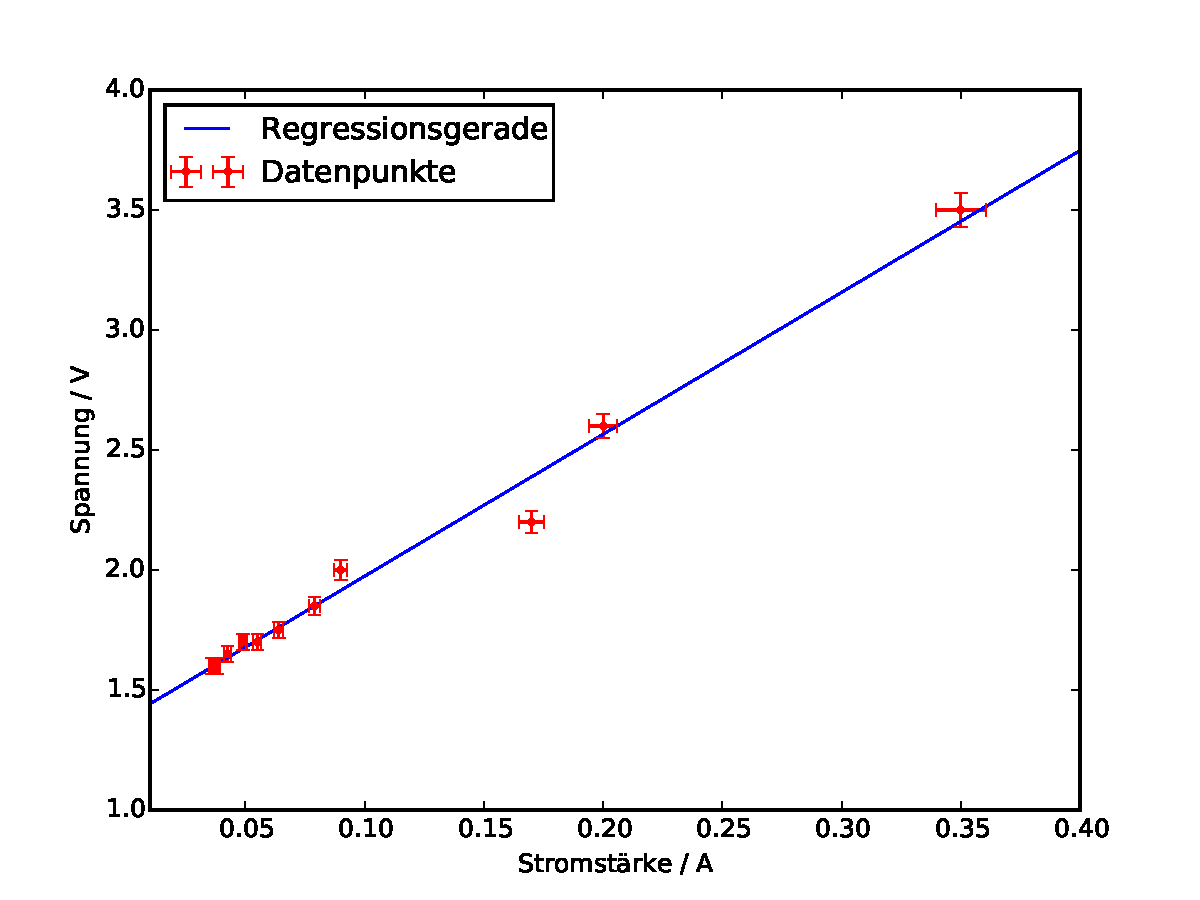
\includegraphics[width=0.95\textwidth]{Spannung_Messung_c.pdf}
	\caption{Lineare Regression zur Gegenspannung}
	\label{fig:Regression_Gegenspannung}
\end{figure}


Für den RC-Generator wird der gleiche Aufbau (siehe Abbildung \ref{Klemmspannung_Bild}) wie bei der Monozelle verwendet. Die Regression ergibt für die Rechteckspannung
\begin{align}
&U_0 = \SI{0.555(6)}{\volt} \ , \\
&R_i = \SI{61.4(19)}{\ohm} 
\end{align}
und für die Sinusspannung
\begin{align}
&U_0 = \SI{0.2332(15)}{\volt} \ , \\
&R_i = \SI{675.6(125)}{\ohm} \ .
\end{align}







\begin{figure}[h!]
	\centering
	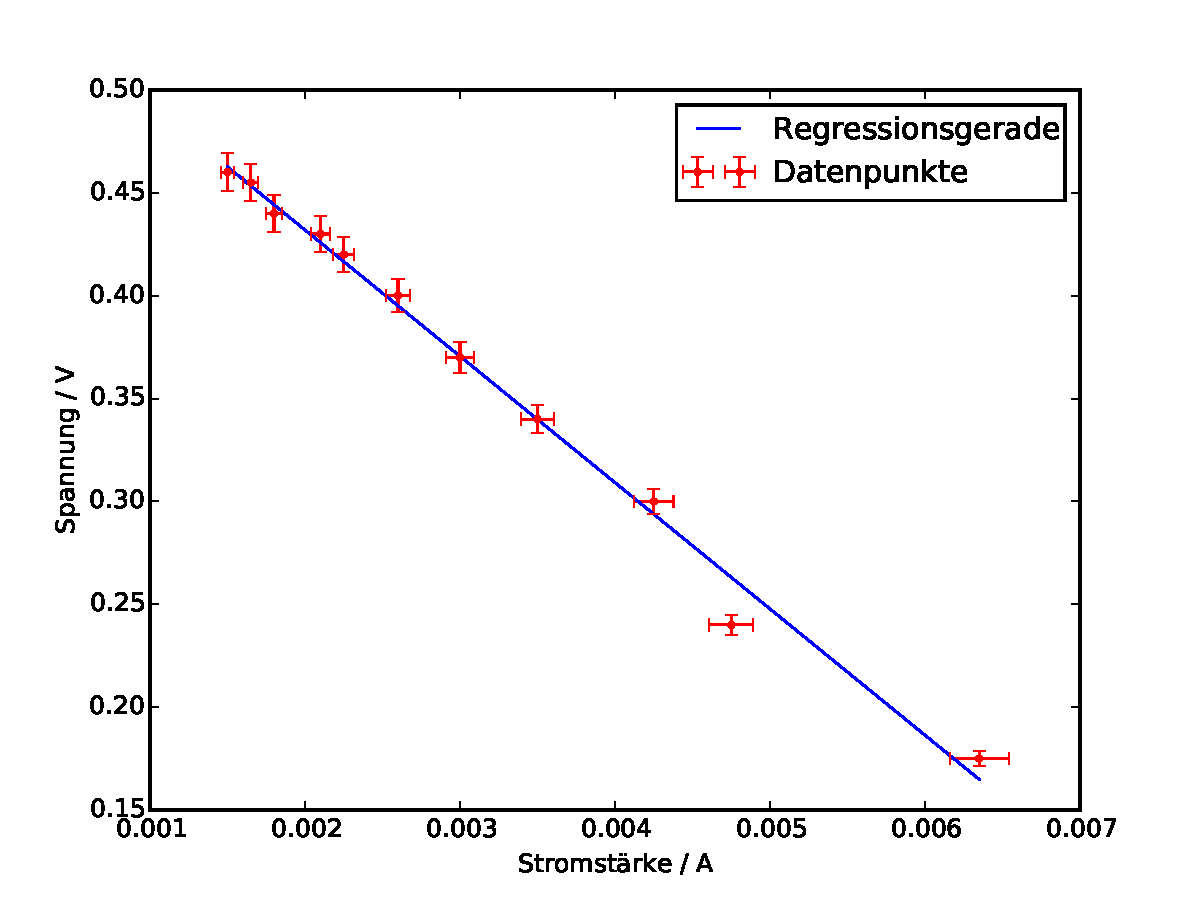
\includegraphics[width=0.95\textwidth]{Spannung_Messung_d.pdf}
	\caption{Lineare Regression zum RC-Generator (Rechteckspannung)}
	\label{fig:Regression_Rechteck}
\end{figure}

\begin{figure}[h!]
	\centering
	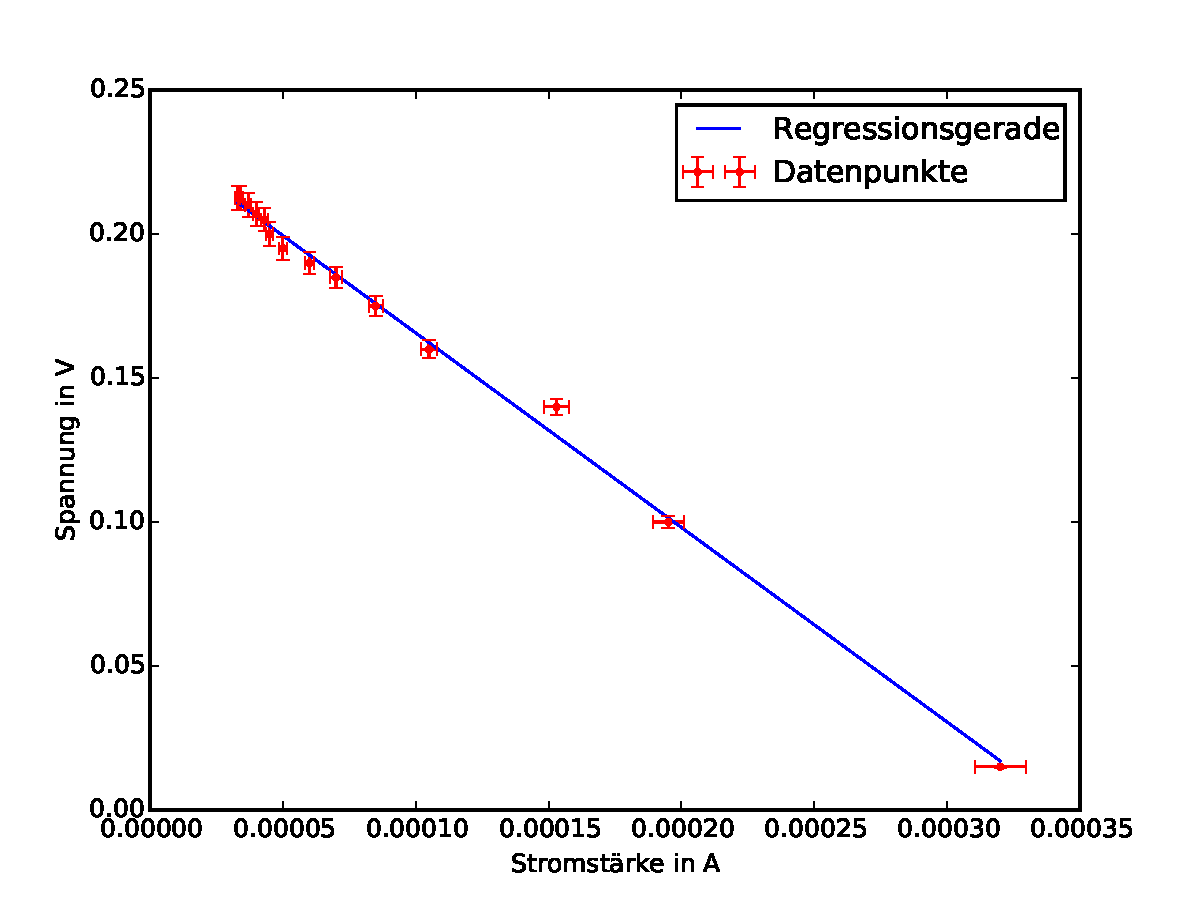
\includegraphics[width=0.95\textwidth]{Spannung_Messung_e.pdf}
	\caption{Lineare Regression zum RC-Generator (Sinusspannung)}
	\label{fig:Regression_Sinus}
\end{figure}

\clearpage

\subsection{Systematischer Fehler -- endlicher Widerstand des Voltmeters}
Der endliche Widerstand des Voltmeters führt zu einem systematischen Fehler. Der Widerstand des Messgerätes müsste unendlich groß sein, um den Stromkreis und -fluss nicht zu beeinflussen. Um den dadurch verursachten Fehler auszurechnen wird die Leerlaufspannung der Monozelle
\begin{equation}
U_k = \SI{1.5}{\volt}
\end{equation}
direkt gemessen.
Der Innenwiderstand der Monozelle (siehe \eqref{Innenwiderstand_Monozelle}) wird aus einer anderen Messreihe übernommen. Durch Umstellen der Formel \eqref{Klemmspannung} nach $U_0$ vereinfacht sich der absolute Fehler zu 
\begin{equation}
\Delta U = U_0 - U_k = I\cdot R_i = U_k \cdot \frac{R_i}{R_v} = \SI{8.191e-7}{\volt}
\end{equation}
und der relative Fehler wird 
\begin{equation}
\frac{\Delta U}{U_k} = \frac{R_i}{R_v} = \SI{5.461e-7}{\%} \ .
\end{equation}
Dieser Fehler ist vernachlässigbar klein.
 
\clearpage 
 
\subsection{Das Maximum der umgesetzten Leistung}
Wie bereits in der Theorie erklärt, ist die umgesetzte Leistung abhängig vom Lastwiderstand $R_a$ und nimmt sogar ein lokales Maximum ein. Hier werden die Messreihen der Monozelle betrachtet. Die Leistung $N_\text{Mess} = U_k \cdot I $ wird über den Belastungswiderstand $R_a = U_k / I$ aufgetragen. Ein Fehler entsteht durch die Ableseungenauigkeit der Messgeräte.

\begin{center}
	\captionof{table}{Belastungswiderstand und Leistung mit Fehlern}
\begin{tabular}{c|c||c|c}
Widerstand in $\si{\ohm}$ & Fehler in $\si{\ohm}$ & Leistung in $\si{\watt}$ & Fehler in $\si{\watt}$ \\
\hline
  0.36  & 0.013  & 0.0225   & 0.00081  \\
  5.21  & 0.188  & 0.1022   & 0.00368  \\
  9.00  & 0.324  & 0.0900   & 0.00325  \\
 15.75  & 0.568  & 0.0840   & 0.00303  \\
 21.70  & 0.782  & 0.0610   & 0.00220  \\
 27.11  & 0.978  & 0.0549   & 0.00198  \\
 32.05  & 1.156  & 0.0488   & 0.00176  \\
 37.50  & 1.352  & 0.0434   & 0.00156  \\
 43.33  & 1.562  & 0.0390   & 0.00141  \\
 49.07  & 1.769  & 0.0358   & 0.00129  \\
 50.96  & 1.837  & 0.0345   & 0.00124  \\
\end{tabular}
\label{Werte_Leistung}
\end{center}

Abbildung \ref{fig:Werte_Leistung} zeigt die theoretische Abhängigkeit der Leistung vom Widerstand (siehe \eqref{Leistung}) und die Werte aus Tabelle \ref{Werte_Leistung}.

\begin{figure}[h!]
	\centering
	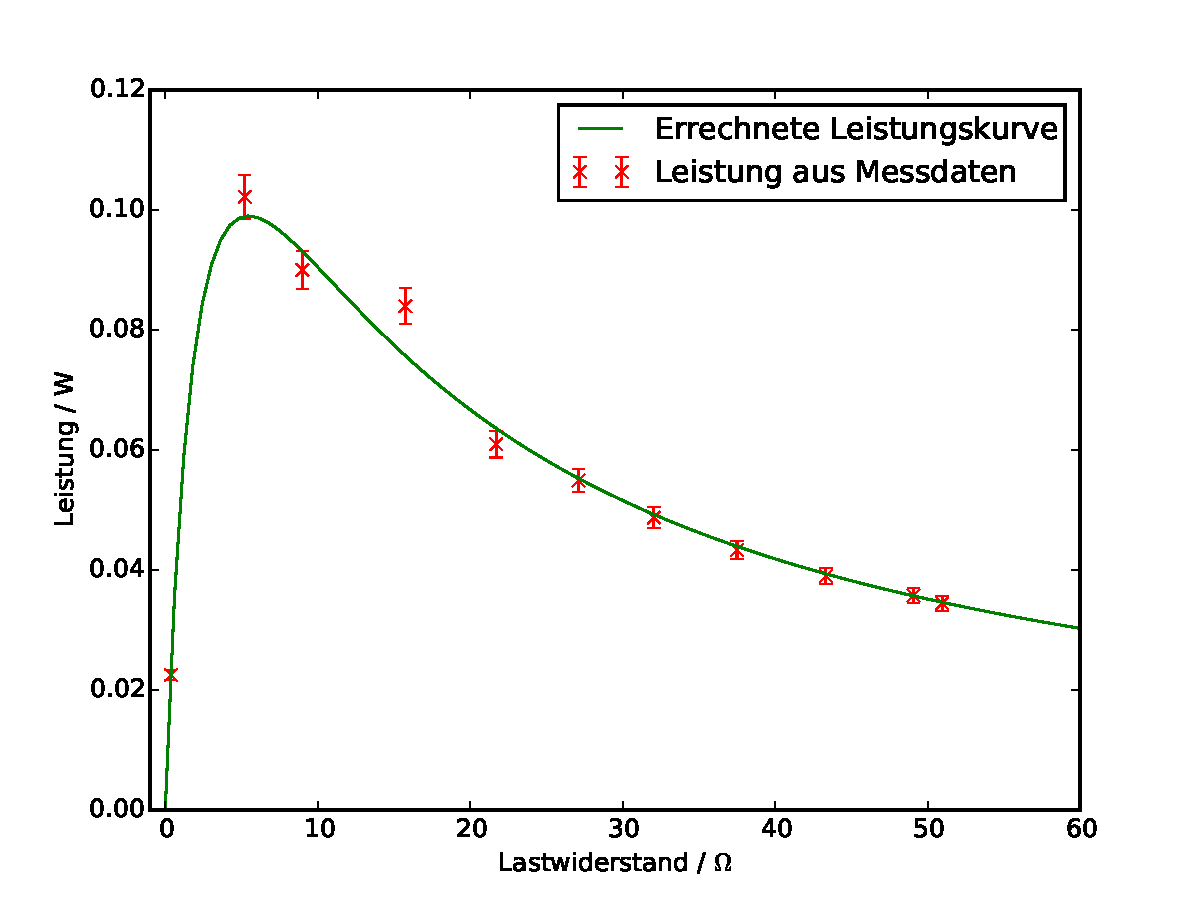
\includegraphics[width=0.95\textwidth]{Leistungskurve.pdf}
	\caption{Leistung $N(R_a)$ am Lastwiderstand}
	\label{fig:Werte_Leistung}
\end{figure}





% R_v????


